123. \begin{figure}[ht!]
\center{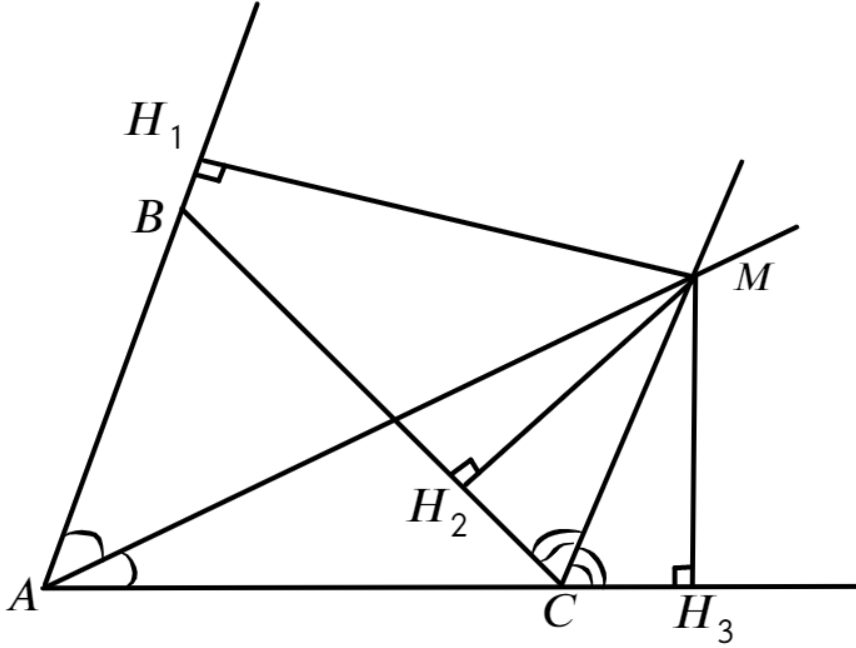
\includegraphics[scale=0.35]{g8-123.png}}
\end{figure}\\
Опустим перпендикуляры $MH_1,\ MH_2$ и $MH_3.$ Тогда по гипотенузе (общей) и углу равны следующие пары треугольников: $MCH_2$ с $MCH_3$ и $MCH_1$ с $MCH_3.$ Тогда $MH_1=MH_3=MH_2=4.$\newpage\noindent
